\chapter{Proposed solution}
\paragraph{}
We have picked SQM as the base for our algorithm. The main factors in this decision were that SQM is faster, produces smaller number of triangles, has better edge flow and even without smoothing the generated mesh better resembles the input skeleton. By avoiding the smoothing phase we do not need any input parameters to generate base mesh from an input skeleton. In this chapter we will explain each step of our proposed algorithm as well as extensions like elliptical nodes, cycles, etc.

\section{Skeleton straightening}
\paragraph{}
Skeleton straightening is a preprocessing step that simplifies bridging of branch node polyhedrons. Straightened skeleton is a skeleton, which nodes in every path between two branch nodes, two leaf nodes, or a branch node and a leaf node are co-linear. Also we have added an extra quality, that angles between branch nodes child nodes should be the same in straightened skeleton, as they are in the input skeleton. To achieve the first condition for each connection node we take the direction of a vector, formed by connection nodes parents position and connection nodes position. The direction vector can be seen in Figure \ref{fig:straightening_ilu} as the green arrow. Then we normalize the direction vector and multiply it by the distance between connection node and its child node. The distance is marked by the black curve in Figure \ref{fig:straightening_ilu}. This vector represents the offset form connection nodes position, at which lies the straightened position of its child node. We then calculate rotation between connection nodes child original position and its new position, in respect to connection nodes position. Finally we rotate all descendants of the connection node. In order to conform to the second condition, at each branch node we do not alter the position of its child nodes.

\begin{figure}[h]
    \centering
    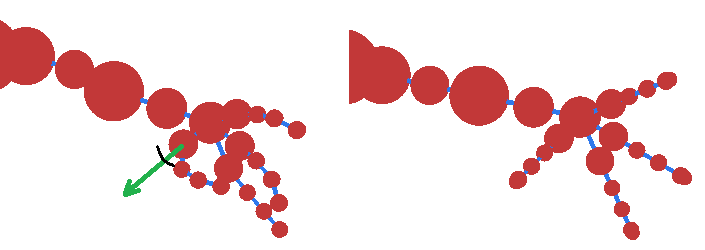
\includegraphics[width=\textwidth]{images/straightening2.png}
    \label{fig:straightening_ilu}
    \caption[Skeleton straightening]{Skeleton straightening; Left: input skeleton, green arrow represents the direction from connection nodes parents position to connection nodes position, black curve marks the distance between connection node and its child; Right: straightened skeleton}
\end{figure}

\subsection{Skinning matrices}
\paragraph{}
In final vertex placement we need to undo the rotations applied to the input skeleton during straightening. We have decided that the best solution is to use skinning, since it can be implemented on GPU and we wanted to move all post-processing on the GPU. Straightened skeleton represents bind pose for skinning purposes and the input skeleton represents reference pose. Now we can calculate skinning matrices required to transform bind pose to reference pose. Traditionally that would require to find the rotation between two corresponding nodes in respect to they parent. Rotating all child nodes in bind skeleton using the same rotation and propagate the rotation calculation to child nodes. But since we know precisely how bind pose was constructed, we can exploit this knowledge and avoid the rotation of child nodes. In fact we do not even need the bind skeleton itself.

\paragraph{}
This can be seen in Figure \ref{fig:DoF_estimation_ilu}. We want to calculate the rotation that would transform circle node to reference pose. We know that circle nodes parent square node is already in reference pose. We also know, that bind pose was constructed in such a way that all connection nodes childes are co-linear and preserve the distances between nodes. That means from squares reference pose we can calculate, where would be circle node, if we would apply on it the same transformation matrices as were applied to square node. The distance between square and circle node remains constant in both poses. And the direction at which the circle node would be is the same as the direction from triangle node to square node, which is marked as green arrow in Figure \ref{fig:DoF_estimation_ilu}. Now we only need to store the rotation between calculated circle node position, green circle in Figure \ref{fig:DoF_estimation_ilu} and its actual position red circle, with respect to its parent red square node.

\begin{figure}[h]
    \centering
    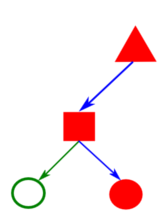
\includegraphics[]{images/DoF_estimation.png}
    \label{fig:DoF_estimation_ilu}
    \caption[Rotation estimation from reference pose]{Rotation estimation from reference pose. Circle: node which rotation we want to estimate; Square: parent of circle node; Triangle: parent of square node; Blue arrows: edges in reference pose; Green circle: circle node position after applying squares skinning matrices; Green arrow: direction from square to green circle node;}
\end{figure}

\section{BNP generation}
\paragraph{}
For each branch node we calculate the direction from said branch node to each of its children and to its parent. Then we create rays, with origin in branch nodes position and direction corresponding to the direction calculated previously. These rays can be seen in Figure \ref{fig:bnp_gen_ilu} (a) as blue arrows. We calculate the intersection of each of these rays with a sphere associated with the branch node. We store each intersection in a set of intersection points. Now we triangulate the intersection points. Different algorithms can be used to achieve the same effect, but we have picked Delaunay triangulation in spherical domain, which was used in the original paper. The algorithm works like standard Delaunay triangulation, but the predicate deciding whatever newly inserted triangle would lie in the circle of an already existing triangle is replaced. The new predicate compares angle between the newly inserted triangles normal with normals of already existing triangles. Result of triangulation is shown in Figure \ref{fig:bnp_gen_ilu} (b) as the blue triangle. The generated polyhedron is now subdivided by inserting a point in the center of each face and in the middle edge. The vertex inserted in the center of each face is then connected with all vertices corresponding to the same face. So each triangle is subdivided into six smaller triangles. The newly inserted points are then projected onto the sphere associated with the node. The subdivision and projection is necessary, because otherwise polyhedrons that would be generated with co-planar, or nearly co-planar intersection points would have no volume or very little volume respectively. To project the newly inserted vertices onto the sphere, we once again use a ray. The origin of the ray is the position of each newly inserted vertex. The direction of the ray is mean normal of the faces that are connected with the vertex. This means that for the vertices in the center of each face the normal of the subdivided face is used. For vertices inserted in the middle of each edge the mean normal of faces corresponding to that edge is used. Final polyhedron is shown in Figure \ref{fig:bnp_gen_ilu} (c).

\begin{figure}[h]
    \centering
    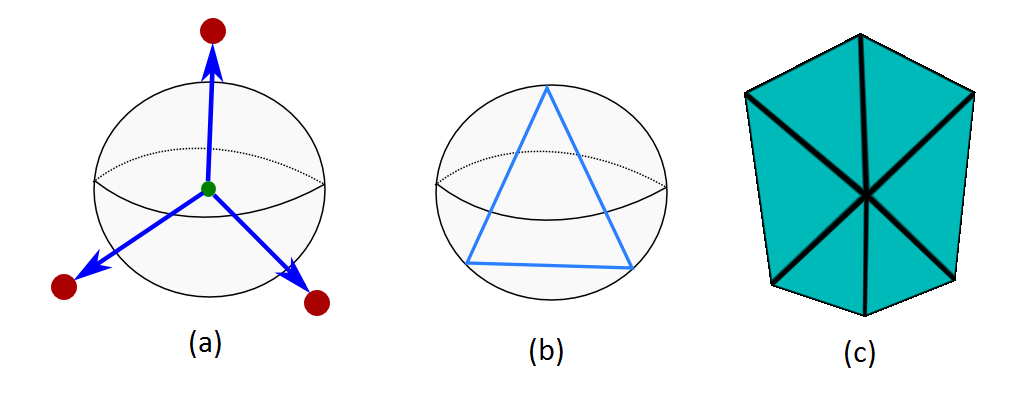
\includegraphics[width=\textwidth]{images/bnp_gen_ilu.png}
    \label{fig:bnp_gen_ilu}
    \caption[BNP generation process]{BNP generation process. (a) green is a branch node, blue arrows represent direction vectors of rays, red circles represent child nodes; (b) blue trinagle is the result of triangulation; (c) final subdivided BNP;}
\end{figure}

\paragraph{}
Triangulation of intersection vertices can sometimes create obtuse triangles. These are problematic, because when we insert the vertex in the middle of an obtuse triangle the one-rings of intersection vertices are not convex. That is if we would project them onto a plane defined by their principal axis and one of the vertices, the resulting polygon would not be convex. In Figure \ref{fig:obtus_tri_ilu} we can see on the left how a polyhedron looks when it is generated with obtuse triangles. Expected central vertex position is marked by red arrow, also expected edges are marked as yellow lines. This is not desirable, since it would cause problems during cyclic mesh generation. To remedy this situation we calculate the projection of the central vertex in a different manner. The origin of its ray is still vertex position. But we use a new direction vector. This vector is the normal of a triangle formed by the projected points that were inserted in the middle of each edge. The result can be seen in Figure \ref{fig:obtus_tri_ilu} on the right.

\begin{figure}[h]
    \centering
    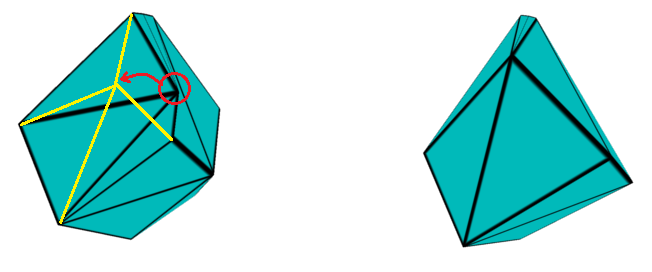
\includegraphics[height=6cm]{images/obtuse_triangle_fix_ilu.png}
    \label{fig:obtus_tri_ilu}
    \caption[Obtuse triangle problem]{Obtuse triangle problem. Left: polyhedron with obtuse triangle. Red arrow marks vertex expected position and yellow lines mark expected edges; Right: polyhedron after applying our fix;}
\end{figure}